\documentclass[12pt,a4paper]{article}

% Quelques options d'encodage, de langues et de format du document
\usepackage[utf8]{inputenc}
\usepackage[T1]{fontenc}
\usepackage[english]{babel}
\usepackage[top=2cm, bottom=3cm, left=1.75cm, right=1.75cm]{geometry}
\usepackage{setspace}
\usepackage{amsmath}
\usepackage{graphicx} % Pour la commande "\includegraphics"
\usepackage{hyperref} % Pour la commande "\url"

\pagenumbering{gobble}

\usepackage{tikz}
\usetikzlibrary{arrows.meta, positioning}

\begin{document}

\begin{center}
  \begin{tabular}{|p{0.2\textwidth}|p{0.75\textwidth}|}
    \hline
    {
    \vspace{0cm} % without it, bugs, don't know why?
    \centerline{\includegraphics[width=\linewidth]{tp-ipp.png}}
    }
    & {
      \vspace{0cm} % same here
      \centering
      \large
      {\hfill January, 2025}
      
      \vspace*{.5cm}
      \textbf{APM\_5AI29\_TP}
      
      \vspace*{.5cm}
      \setstretch{1.5}
      {\Large\textbf{Language Models and Structured Data}}
      
      \vspace*{.5cm}
      Mid-term Project Report

      \vspace*{1cm}
      %{\hfill\href{http://teaching.simplicitytheory.science}{teaching.simplicitytheory.science}}
      } \\
    \hline
  \end{tabular}
\end{center}

\noindent Acronym of the Team: FITJ\\
Name:	Fidelin-Durand Julian, Isabelle Neuveu, Tao Guinot, Florian Morel

{\centering\rule{\linewidth}{.5pt}}


%\maketitle
\begin{center}
\section*{Text To SQL}
\end{center}
\section*{Abstract}

2/3 lines of abstract

\section*{Problem Statement}

Chatting with data has been the most in demand application of LLMs past year, enterprises spending on GenAI increased sixfold in 2024, while it reached \$2.3 billion in 2023, enterprises are now looking for strong ROI and an important part of them are considering improving operation efficiency and data retrieval as the main criteria of investment \cite{MarketAnalysis} \cite{DeloitteResearch}.

Frameworks such as langchain of llama index have made simple to connect with SQL databases to write basic queries. But moving from basic to more advanced queries remain challenging, even more for smaller models adopted on premise by companies. Enterprises are looking for agents which they can chat with. Instead of groing from no automation to full automation (chatting with data directly), it is important to take a look at semi automation to understand what tasks the agent is actually performing, in our case translating a user's query to a SQL query.

Furthermore, breaking down the whole agent process may mitigate associated risks such as operational risks, data privacy risks, security risks or financial risks; being mostly due to the database access and the SQL query execution bypassing the user's correction.
\\

We present here a 3-step method to implement an agent capable at generating SQL queries from a user's question that would be usable in a production pipeline:
\begin{enumerate}
    \item Zero-shot and prompt engineered LLM evaluation (small general models and SQL-pretrained models)
    \item Fine tuned LLM, how good can they generalize ?
    \item Agent-based architecture and Retrieval-Augmented Generation
\end{enumerate}


\section*{Method/Overall Architecture}

As described earlier, our method will consist in 3 steps.
\subsection*{Zero-shot and prompt engineering}

In order to compare different ways to obtain the expected SQL queries, we decided to test two models, one general "Gemini" and one specifically trained to generate code "IBM-Granite". Both are given the schema and a prompt as inputs.
\\
We also chose two approaches: the zero-shot prompt and the few-shot prompt, to witness if it makes any difference for the models. As an example of engineered prompts we have:\\
\\
- Zero-shot prompt: \\
\\
"Reply the SQL query only, without any comment, using this schema stadium : Stadium ID (number) , Location (text) , Name (text) , Capacity (number) , Highest (number) , Lowest (number) , Average (number) | singer : Singer ID (number) , Name (text) , Country (text) , Song Name (text) , Song release year (text) , Age (number) , Is male (others) | concert : concert ID (number) , concert Name (text) , Theme (text) , Stadium ID (text) , Year (text) | singer in concert : concert ID (number) , Singer ID (text)' to the question: How many singers do we have?
SQL QUERY:"\\
\\
- Few-shot prompt: \\
\\
"Reply only the SQL query, using this schema stadium : Stadium ID (number) , Location (text) , Name (text) , Capacity (number) , Highest (number) , Lowest (number) , Average (number) | singer : Singer ID (number) , Name (text) , Country (text) , Song Name (text) , Song release year (text) , Age (number) , Is male (others) | concert : concert ID (number) , concert Name (text) , Theme (text) , Stadium ID (text) , Year (text) | singer in concert : concert ID (number) , Singer ID (text)', the same way as in the examples below:\\
-----------\\
EXAMPLES\\
Question: What is the 3 most common cloud cover rates in the region of zip code 94107?
SELECT cloud cover FROM weather WHERE zip code  =  94107 GROUP BY cloud cover ORDER BY COUNT (*) DESC LIMIT 3\\
Question: Count the number of schools.\\
 SELECT count(*) FROM school\\
Question: What are the names of all campuses located at Chico?\\
 SELECT campus FROM campuses WHERE LOCATION  =  "Chico"\\
Question: Which colleges does each player with a name that starts with the letter D  who tried out go to?
 SELECT T1.cName FROM  tryout AS T1 JOIN player AS T2 ON T1.pID  =  T2.pID WHERE T2.pName LIKE 'D\%'\\
Question: What are the names of all the players who received a yes during tryouts, and also what are the names of their colleges?\\
 SELECT T1.pName ,  T2.cName FROM player AS T1 JOIN tryout AS T2 ON T1.pID  =  T2.pID WHERE T2.decision  =  'yes'\\
-----------\\
QUESTION: What is the average, minimum, and maximum age for all French singers?\\
SQL QUERY:"\\
\subsection*{Fine-Tuning LLM}

- Explain how to fine tune them:
What to give ? SQL Schema, should we re arrange the schema description to be more comprehensive for the LLM ? Mask training ?

\subsection*{Agent-based architecture}

An agent is an object aiming at choosing a sequence of actions to take. In chains, those actions are hardcoded while agents use language models to determine which action to take and in which order. A agent built to interact with databse would look like this:

\begin{itemize}
    \item Itent classification is performed to better understand the user's query
    \item Text-to-SQL is often framed as Retrieval-Augmented Generation application, where context (table schema, examples queries, etc.) are retrieved to enhance the performance of the LLM to answer the question. 
    \item A set of validators can be ran followed by a self-correction agent to fix errors.
\end{itemize}

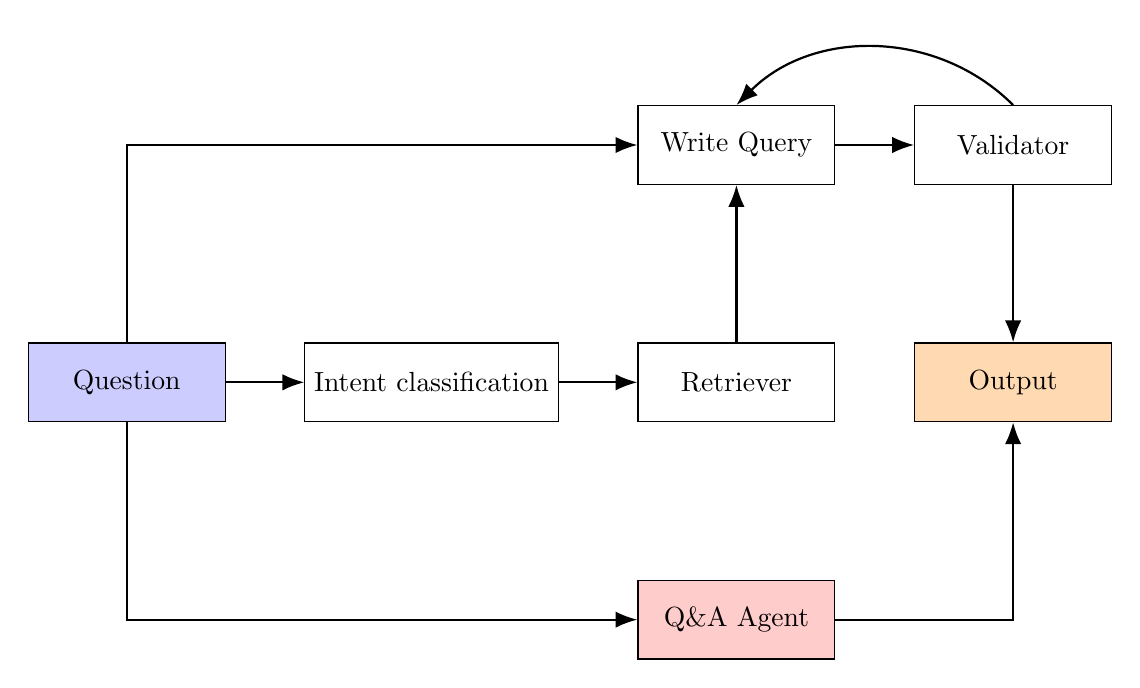
\begin{tikzpicture}[
    node distance=2cm and 1cm,
    every node/.style={draw, align=center, minimum width=2.5cm, minimum height=1cm},
    arrow/.style={-{Latex[scale=1.2]}, thick}
]

% Nodes
\node (question) [fill=blue!20] {Question};
\node (classification) [right=of question] {Intent classification};
\node (retriever) [right=of classification] {Retriever};
\node (writequery) [above=of retriever] {Write Query};
\node (validator) [right=of writequery] {Validator};
\node (output) [below=of validator, fill=orange!30] {Output};
\node (qanda) [below=of retriever, fill=red!20] {Q\&A Agent};

% Arrows
\draw [arrow] (question) -- (classification);
\draw [arrow] (classification) -- (retriever);
\draw [arrow] (retriever) -- (writequery);
\draw [arrow] (writequery) -- (validator);
\draw [arrow] (validator) -- (output);

% Edge arrows with 90° angles
\draw [arrow] (question.north) -- ++(0,0.5) |- (writequery.west);  % Arrow to Write Query
\draw [arrow] (question.south) -- ++(0,-0.5) |- (qanda.west);     % Arrow to Q&A Agent
\draw [arrow, bend right=45] (validator.north) to (writequery.north); % Bended arrow

% Arrow with 90° angle from Q&A Agent to Output
\draw [arrow] (qanda.east) -| (output.south); % 90° angle arrow (right then up)

\end{tikzpicture}

It is important to mention that because some table can be incomplete or doesn't necessarily contain explicit column names, a certification effort has to be pursued to describe the databases. Those description can consist in human description of table and their fields, an AI description, jargon, query examples or description status.

Since this is not the aim of our work, we will focus on building a simpler yet effective agent.
\vspace{1cm}

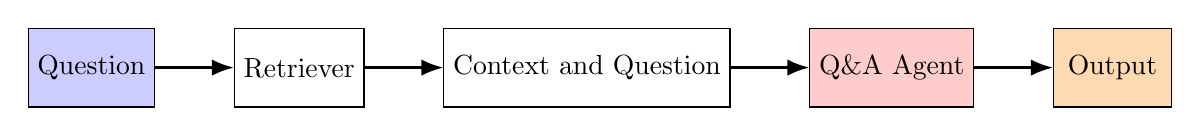
\begin{tikzpicture}[
    node distance=1cm and 1cm,
    every node/.style={draw, align=center, minimum width=1.5cm, minimum height=1cm},
    arrow/.style={-{Latex[scale=1.2]}, thick}
]

% Nodes
\node (question) [fill=blue!20] {Question};
\node (retriever) [right=of question] {Retriever};
\node (contextquestion) [right=of retriever] {Context and Question};
\node (qanda) [right=of contextquestion, fill=red!20] {Q\&A Agent};
\node (output) [right=of qanda, fill=orange!30] {Output};


% Arrows
\draw [arrow] (question) -- (retriever);
\draw [arrow] (retriever) -- (contextquestion);
\draw [arrow] (contextquestion) -- (qanda);
\draw [arrow] (qanda) -- (output);

\end{tikzpicture}

\subsection*{Evaluation}
The goal is to produce a SQL query as close as a groundtruth query provided in a train dataset. It is important to notice that two different queries can lead to the same result with different performance when ran toward a SQL database.

To evaluate the LLM performance, we set different metrics:
\begin{enumerate}
    \item Keyword metric
    \item Identifier metric
    \item Logical metric
\end{enumerate}
\\
Let us review those metrics.

\subsubsection*{Keyword metric}

The \texttt{keyword\_score} is a metric that evaluates the similarity between the keywords of two SQL queries (the predicted query and the ground truth query). It is based on the F1 score, which measures the balance between precision and recall. The formula for the F1 score is given by:

\[
\text{F1 score} = \frac{TP}{TP + 0.5 \times (FP + FN)}
\]

Where:

\begin{itemize}
  \item \( TP \) (True Positives) is the number of keywords that appear in both the predicted query and the ground truth query.
  \item \( FP \) (False Positives) is the number of keywords present in the predicted query but not in the ground truth query.
  \item \( FN \) (False Negatives) is the number of keywords present in the ground truth query but not in the predicted query.
\end{itemize}

The \texttt{keyword\_score} is computed as follows:
\[
\text{keyword\_score} = \text{F1 score}(keywords_{\text{pred}}, keywords_{\text{gt}})
\]
Where \( keywords_{\text{pred}} \) and \( keywords_{\text{gt}} \) are the sets of keywords extracted from the predicted and ground truth SQL queries, respectively.

The \texttt{keyword\_score} ranges from 0 to 1:
\begin{itemize}
  \item A score of 1 indicates perfect overlap in the keywords between the predicted and ground truth queries.
  \item A score of 0 indicates no overlap in keywords.
\end{itemize}

\subsubsection*{Identifier metric}

The \texttt{identifier\_score} is a metric that compares the identifiers (such as table names and column names) between the predicted SQL query and the ground truth query. It is calculated by computing the F1 score for identifiers for each common keyword between the two queries. The steps are as follows:

\begin{enumerate}
    \item Identify common keywords between the predicted query and the ground truth query.
    \item For each common keyword, retrieve the identifiers associated with that keyword in both queries.
    \item Compute the F1 score for the identifiers of the predicted and ground truth queries for each keyword:
    \[
    \text{F1}_{\text{identifier}}(k) = \frac{TP_k}{TP_k + 0.5 \times (FP_k + FN_k)}
    \]
    where:
    \begin{itemize}
        \item \( TP_k \) is the number of identifiers common between the predicted and ground truth queries for keyword \( k \).
        \item \( FP_k \) is the number of identifiers in the predicted query but not in the ground truth for keyword \( k \).
        \item \( FN_k \) is the number of identifiers in the ground truth query but not in the predicted query for keyword \( k \).
    \end{itemize}
    \item The final \texttt{identifier\_score} is the average F1 score across all common keywords:
    \[
    \text{identifier\_score} = \frac{1}{|\text{commun\_keywords}|} \sum_{k \in \text{commun\_keywords}} \text{F1}_{\text{identifier}}(k)
    \]
\end{enumerate}

\subsubsection*{Logical metric}




The Logical metric, or \texttt{equivalence\_score} method, is designed to return a numerical score representing how similar a generated SQL query is to a groundtruth query, based on the evaluation of an orchestrator LLM. This score is computed by invoking a separate model that compares the two queries and returns a score.
\\
\\
\textbf{Parameter}
\begin{itemize}
    \item \texttt{generated\_query}: A SQL query generated by the model based on a user's question.
    \item \texttt{query}: The groundtruth SQL query, which serves as the reference for comparison.
    \item \texttt{score\_prompt}: A prompt template used to ask the orchestrator LLM to provide a score.
\end{itemize}
\\
\textbf{Explanation}
\\
The method is aiming at returning a score between 0 and 1 and give some explanation of the result. The numerical score is found from the LLM answer with the regular expression pattern \texttt{\textbackslash s*([0-9]*\.?[0-9]+)}.
\\

\textbf{Return Values}
\\
The method returns a tuple containing:
\begin{itemize}
    \item A \texttt{float} representing the equivalence score between the two queries.
    \item A \texttt{str} explaining the score, which might include further details about the comparison.
\end{itemize}


score\_prompt = """Determine the degree of logical equivalence between the two SQL queries, assuming the same schema, data, and execution environment. Provide a score between 0 and 1, where:
\\
- 1: Fully logically equivalent (queries produce identical results under all circumstances).
\\
- 0: Completely different (queries are logically unrelated or produce entirely different results).
\\
- Scores between 0 and 1 should reflect partial equivalence, considering factors such as:
\\
- Differences in filters, conditions, or joins that partially overlap.
\\
- Minor variations in selected columns or formatting that do not affect the overall logic.
\\
- Similar intent but differing specifics in query structure.
\\
Explain your score briefly, highlighting key differences or similarities that influenced the rating.
Query 1:
\{query\}
Generated query:
\{generated\_query\}
Equivalence Score (0-1, with explanation):"""






\section*{Experimentation}
\subsection*{Results for Zero-shot and prompt engineering}

- Give some results obtained


\begin{itemize}
\item Dataset \& Dataset Statistics
\item Experimental Results based on Evaluation Metrics
\item Error Analysis
\end{itemize}

\section*{Discussion}

Comparison with expectations, limitations, lessons learned, and perspectives.

\section*{Bibliography}
\bibliographystyle{plain}
\bibliography{sample}


\end{document}
